\documentclass{article}
\usepackage[classica]{topfront}
\usepackage[utf8]{inputenc} %utf8
\usepackage[english]{babel}
\usepackage[T1]{fontenc}
\usepackage{blindtext}
\usepackage{graphicx,wrapfig}
\usepackage{booktabs}
\usepackage{lmodern}
\usepackage{physics}
\usepackage{varioref}
\usepackage{url}
\usepackage{array}
\usepackage{paralist}{\obeyspaces\global\let =\space}
\usepackage{verbatim}
\usepackage{subfig}
\usepackage{tabularx}
\usepackage{amsmath}
\usepackage{accents}
\usepackage{slashed}
\usepackage{amsfonts}
\usepackage{float}
\usepackage{amssymb}
\usepackage{multicol}
\usepackage{multirow}
\usepackage{listings}
\usepackage[a4paper, total={5.5in, 8in}]{geometry}
\usepackage[figuresright]{rotating}
\usepackage{algorithm}
\usepackage{algpseudocode}
\usepackage{amsmath}
\usepackage{physics}
\usepackage{bbold}
\usepackage[babel]{csquotes}
\usepackage{hyperref}
\usepackage{braket}
\usepackage{mathtools}
\usepackage{subfig}
\usepackage{setspace}
\usepackage[sorting=none,style=numeric-comp,backend=biber]{biblatex}
\usepackage{tikz}
\usepackage{mathdots}
\usepackage{yhmath}
\usepackage{cancel}
\usepackage{color}
\usepackage{siunitx}
\usepackage{array}
\usepackage{multirow}
\usepackage{amssymb}
\usepackage{gensymb}
\usepackage{tabularx}
\usepackage{extarrows}
\usepackage{booktabs}
\graphicspath{ {images/} }
\addbibresource{bibliography.bib}

\title{Determination of the critical point in a SU(3) Yang-Mills theory}

\author{Mitsuaki Hirasawa, Luca Virzì}
\begin{document}

\maketitle

From theoretical arguments and empirical evidence, we expect a SU(3) Yang-Mills theory to show a first order transition for a critical temperature $T_c$. In this letter we present the procedure we used to determine the pseudocritical point in the framework of a thermal field theory with shifted boundary conditions. The critical temperature $T_c$, or equivalently the critical coupling $\beta_c$, is retrieved by studying the behaviour of an order parameter for the transition, namely the expectation value of the Polyakov Loop $\langle P \rangle$. Once that the we have found the transition point, we can compute some thermodynamic quantities of interests, such as the latent heat of our system.

\section{Introduction}
A number of different areas of research in Physics would benefit from a deeper phenomenological understanding of the phenomena governing strong-interactions. For instance, it is of cosmological interest to explain the collective behaviour of strongly interacting particles, since the latter determined the evolution of the Universe in its early stages. The study of the Equation of State (EoS) of Quantum Chromodynamics (QCD) could shed some light on strong-interactions phenomenology, hence it is an extremely relevant subject in particle and nuclear physics, moreover it serves as a theoretical input in the analysis of experimental results coming from heavy-ion colliders. %\\

The only theoretical tool which allows us to study the EoS from first principles is given by the regularization of QCD on a discrete four-dimensional hypercube, namely Lattice QCD \cite{Boyd_1996, Bors_nyi_2014, Umeda_2009}, see \cite{Philipsen_2013} for a somewhat dated review. Full QCD results are still scarce today, but we can retrieve useful insights from the study of its so-called quenched limit, namely a theory where $N_f = 0$. 
In this Letter we will work within the framework of a relativistic thermal quantum field theory, i.e. we will consider a SU(3) Yang-Mills theory at a finite temperature $T$, which is a confining gauge theory.

It is widely accepted from theoretical and empirical arguments that quenched QCD undergoes a first order transition at a critical temperature in the order of 290 MeV, associated with the spontaneous breaking of the $Z(3)$ symmetry of the theory \cite{Borsanyi:2022xml}. %with the precise value of $T_c$ being dependent on the particular scale setting choices.
A strong confirmation of the validity of these arguments would be given by the computation of the latent heat of the system, as a non-zero value is associated with a first-order transition with certainty. %\\



In the last decade, new numerical methods based on the formulation of a thermal theory in a moving frame have been developed \cite{Giusti_2014, Giusti_2017}. In this framework, the EoS is investigated through the computation of the entropy density as the primary variable of our simulations, since this quantity is proportional to the total momentum of the system as measured by an observer in a moving frame. This strategy exploits the Poincaré symmetry of the relativistic field theory to derive suitable Ward-Takahashi identities (WIs), which can be easily related to the thermodynamic quantities we are interested in, as shown in
 \cite{Implications, Giusti_2011}. Assuming the reader has familiarity with the cited works, we will briefly recall some useful concepts. Consider the SU(3) Yang-Mills theory defined on a lattice of finite spatial volume $L^3$ and finite temporal extension $L_0$. Adopting the Euclidean metric, we can write the partition function of the system in a moving frame with imaginary velocity $\vb*{v} = i\vb*{\xi}$ as:
\begin{equation}
    Z = \Tr{e^{-L_0(\hat{H} - i \vb*{\xi} \cdot \vb*{\hat{P}})}}
\end{equation}
Its Euclidean path integral formulation can be derived in the usual manner by imposing periodic boundary conditions in the spatial direction and shifted boundary conditions along the compact direction:
\begin{equation}
    \phi(L_0, \vb*{x}) = \phi(0, \vb*{x} - L_0 \vb*{\xi})
\end{equation}
where $\phi$ is a generic field and $\vb*{\xi} = (\xi_1, \xi_2, \xi_3)$ is the shift in the spatial directions. Notice that, due to spatial periodicity, $\xi_k' = \xi_k + L/L_0$, and therefore the single components of the shift are restricted to the interval:
\begin{equation}
    - \frac{L}{2L_0} \le \xi_k \le \frac{L}{2L_0}
\end{equation}
In the Euclidean formulation, the system dynamics is invariant under SO(4) rotations, which in turn implies the following relation for the free energy of the system:
\begin{equation}
    f(L_0, \vb*{x}) = f\left(L_0 \sqrt{1 + \vb*{\xi}^2}, 0\right)
\end{equation}
which consequently depends on the combination $L_0 \sqrt{1 + \vb*{\xi}^2} = T^{-1}$, i.e. the inverse of the temperature of the system, rather than $L_0$ and $\vb*{\xi}$ separately. %\\
From this observation it follows that the total momentum and energy distribution are related through some interesting WIs, which can be exploited for the computation of thermodynamic quantities. For instance one can show \cite{Giusti_2011, Giusti_2014, Giusti_2017, Implications} that the entropy density can be written as:
\begin{equation}
    \frac{s(T)}{T^3} = - \frac{(1 + \vb*{\xi}^2)}{\xi_k}\frac{\langle T_{0k} \rangle_{\vb*{\xi}}}{T^4}
\end{equation}
where $\langle \cdot \rangle_{\vb*{\xi}}$ stands for an expectation value in presence of a non-zero shift $\vb*{\xi}$, and $T_{0k}$ is an off-diagonal component of the energy-momentum tensor. %\\

The numerical strategy connected with this formulation of the thermal theory in a moving frame avoids the technical difficulties associated with the standard numerical methods, based on the direct measurement of the trace anomaly through Monte Carlo simulations. Typically the latter are more numerically demanding due to the ultra-violet power divergences one has to take care of, on contrary to what happens in our case, where for instance $\langle T_{0k} \rangle_{\vb*{\xi}}$ does not need any ultra-violet subtraction.
\\ The rest of this Letter is structured as follows: in Section 2 ...

\section{Critical point}
In this section we will focus on the localization of the critical point of the theory, before moving on to the computation of the latent heat. The SU(3) Yang-Mills gauge theory is regularized on a four-dimensional hypercube of finite spatial volume $V = L^3$, temporal extension $L_0$ and lattice spacing $a$. Gauge fields are represented by link variables $U_\mu(x) \in SU(3)$, which satisfy periodic boundary conditions in the spatial direction and shifted boundary conditions along the temporal one:
\begin{equation}
    U_\mu(L_0, \vb*{x}) = U_\mu(0, \vb*{x} - L_0 \vb*{\xi
})
\end{equation}
where $(L_0/a) \, \vb*{\xi}$ is a vector with integer components. Up to a constant, the Wilson action is given by:
\begin{equation}
S[U] = \frac{3}{g_0^2} \sum_x \sum_{\mu, \nu} \left[1 - \frac{1}{3} \Re \Tr{U_{\mu\nu}(x)} \right]
\end{equation}
where the trace is taken over the color index, $g_0$ is the bare coupling and $U_{\mu\nu}(x)$ is the standard plaquette:
\begin{equation}
    U_{\mu\nu}(x) = U_\mu(x)U_\nu(x + a\hat{\mu})U_\mu^\dagger(x + a\hat{\nu})U_\nu^\dagger(x)
\end{equation}
with $\mu, \nu = 0, \dots, 3$, $\hat{\mu}$ being the unit vector along the corresponding direction, and $x$ the space-time coordinate. 
To generate gauge configurations in our simulation, we adopt the heatbath and overrelaxation updating scheme, accordingly to the Cabibbo-Marinari algorithm \cite{Cabibbo:1982zn}.%\\

A $SU(3)$ Yang-Mills theory with static quarks, the so-called quenched approximation of QCD, shows a first-order deconfining transition, associated with the spontaneous breaking of the global $Z(3)$ symmetry of the system at some critical temperature. %\\
We will localize the transition point following the procedure described in Ref. \cite{Francis_2015}, namely we adopt a statistical-physics method where finite-volume effects are exponentially suppressed. 
The procedure is the following.%\\

The expectation value of the Polyakov loop is a good order parameter for the identification of the breaking of the $Z(3)$ symmetry, and it is defined as:
\begin{equation}
    \langle P \rangle = \frac{1}{V} \langle \Tr\prod_{x_0 = 1}^{N_\tau} U_0(x_0, \vb*{x}) \rangle
\end{equation}
where $N_\tau$ is the number of lattice sites in the time direction. %\\
To localize the transition point, we first notice that the vacuum in the confined phase has no-degeneracy, while in the deconfined phase the $Z(3)$ center symmetry implies a 3-fold degeneracy. During a sufficiently long Monte Carlo history, we expect to observe tunneling events between these four vacua, as one can see from the distribution of $\langle P \rangle$ in Figure \ref{fig:P2d}. %\\
\begin{figure}[htbp]
    \centering
    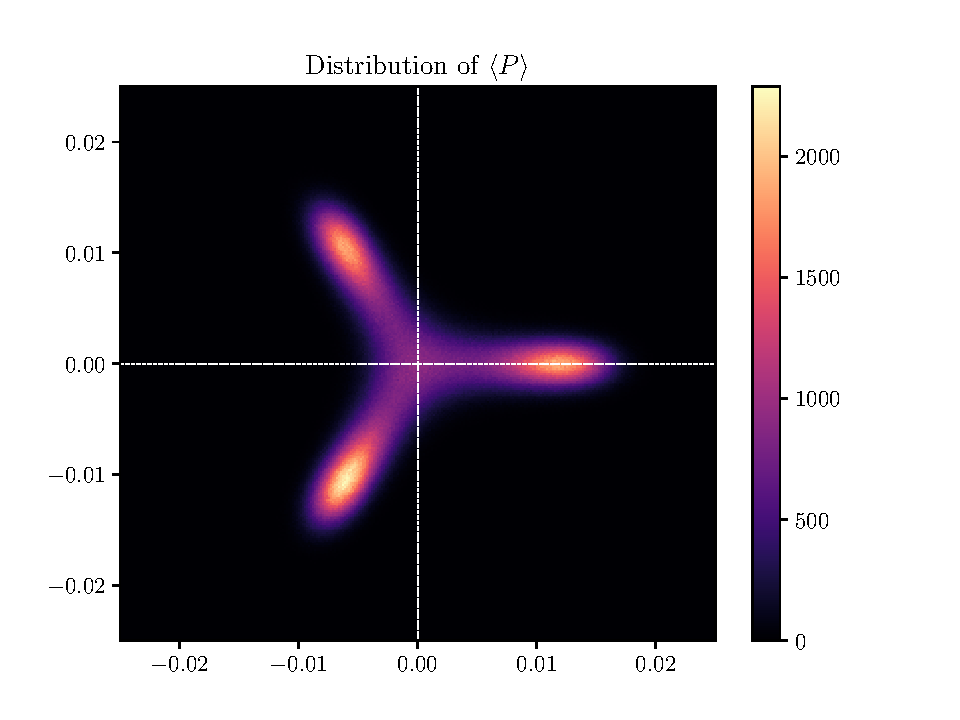
\includegraphics[width=0.8\linewidth]{imgs/P_run2.pdf}
    \caption{Distribution of $\langle P \rangle$ for $\beta = 6.1025$ at $L_0=6$, close to the transition point.}
    \label{fig:P2d}
\end{figure}
Given a criterion to separate the confined and deconfined phases, we can define the weights $w_c$ and $w_d$ as the volume of the distribution of $\langle P \rangle$ in the respective phases, which allow us to build a parameter that signals the occurance of the transition:
\begin{equation}
    s(\beta) = \frac{3w_c - w_d}{3w_c + w_d}
\end{equation}
Indeed, we have $s(\beta) = 1$ deep in the confined phase ($w_d = 0$), $s(\beta) = -1$ deep in the deconfined phase ($w_c = 0$) and $s(\beta) = 0$ at the transition point, where $w_d = 3w_c$. %\\

The technique we adopted to separate the two phases is based on the localization of a local minimum in the distribution of the real part of the Polyakov loop expectation value. For the sake of simplicity, since the three degenerate vacua in the deconfined phase are equivalent, we perform a rotation on the spectrum of $\langle P \rangle$ to overlap the latter. The resulting distribution shows two peaks associated with each phase, and the local minimum between the peaks will regarded as the border between them, as shown in the example Fig. \ref{fig:distrReP}. %\\
The minimum position is estimated through a quartic fit in the region between the peaks. %\\
Consequently, the weights $w_c$ and $w_d$ are defined respectively as the integral of the distribution of $\Re\langle P \rangle$ under each corresponding peak. %\\
\begin{figure}[htbp]
    \centering
    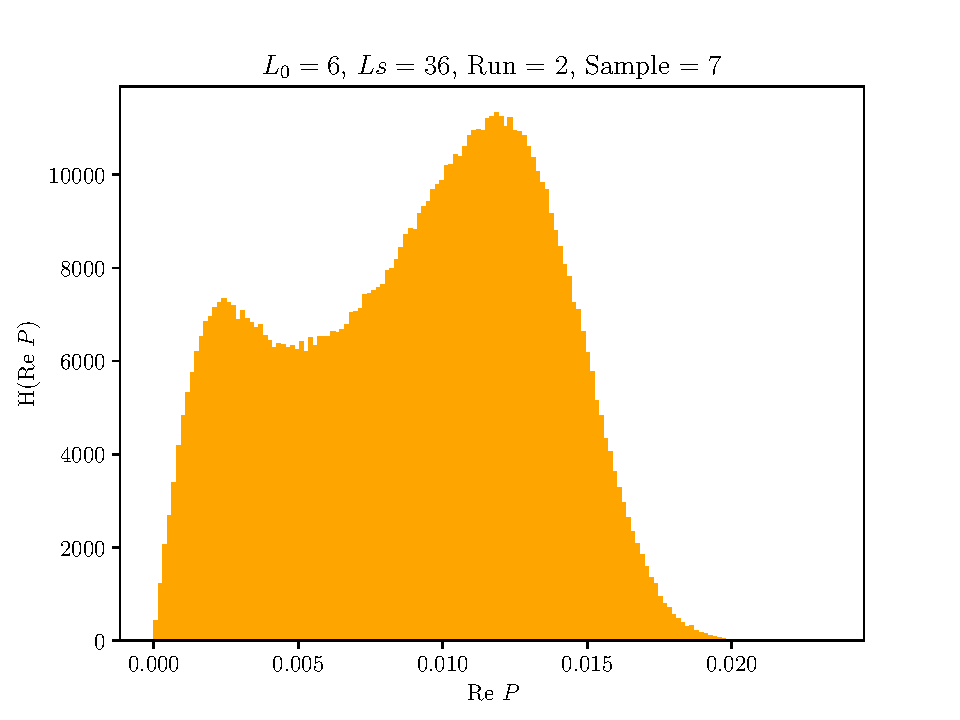
\includegraphics[width=0.3\hsize]{imgs/ReP_run2.pdf}
    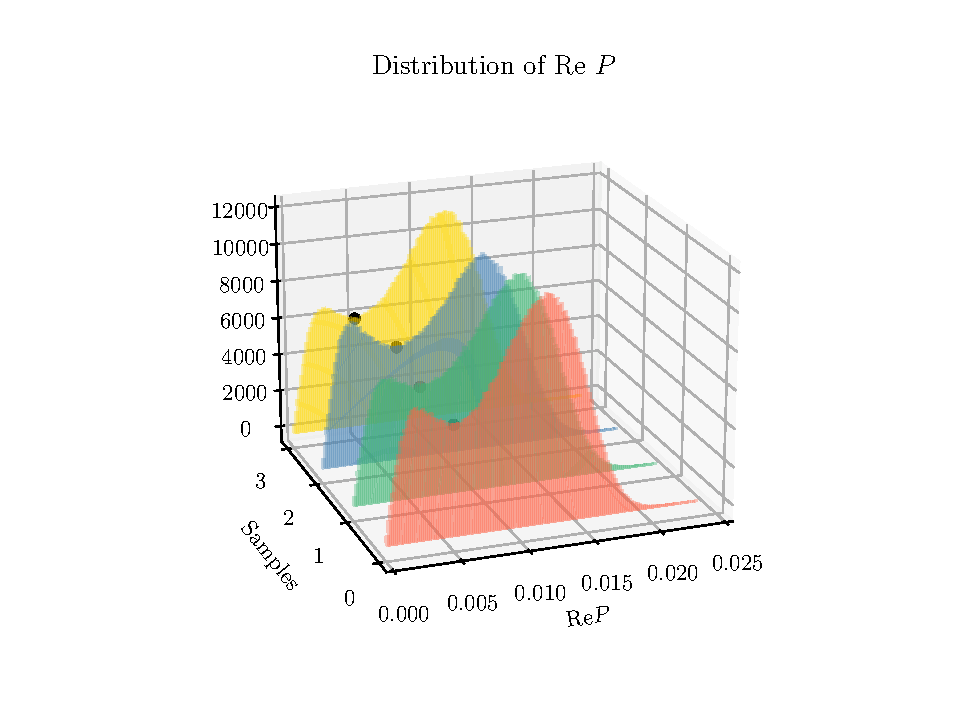
\includegraphics[width=0.4\hsize]{imgs/histograms3d_run2.pdf}

    \caption{(Left) Distribution of $\Re \langle P \rangle$ for $\beta = 6.020$ at $L_0=6$. After the spectrum rotation, the peak structure is clear. 
    (Right) Distribution of $\Re \langle P \rangle$ for different subsamples, $\beta = 6.020$.}
    \label{fig:distrReP}
\end{figure}

In order to perform a statistical analysis of the collected data, we divided our $\langle P \rangle$ dataset into $\mathcal{O}(15)$ subsamples, and for each of the latter we computed $s(\beta)$ by following the steps described above. In Figure \ref{fig:multi-histo} we show the product of this analysis for some subsamples. \\
We carried this analysis out for different lattices, and for each one we have computed $s(\beta)$ for several values of the gauge coupling. Through a linear fit of $s(\beta)$ around the transition point, we can interpolate the critical value $\beta_c$, see Figure \ref{fig:beta-crit10bins} for an example.%, which in our case is $\beta_c = 6.10287(16)$. The fit is reproduced in Figure \ref{fig:beta-crit10bins}.
\begin{figure}
    \centering
    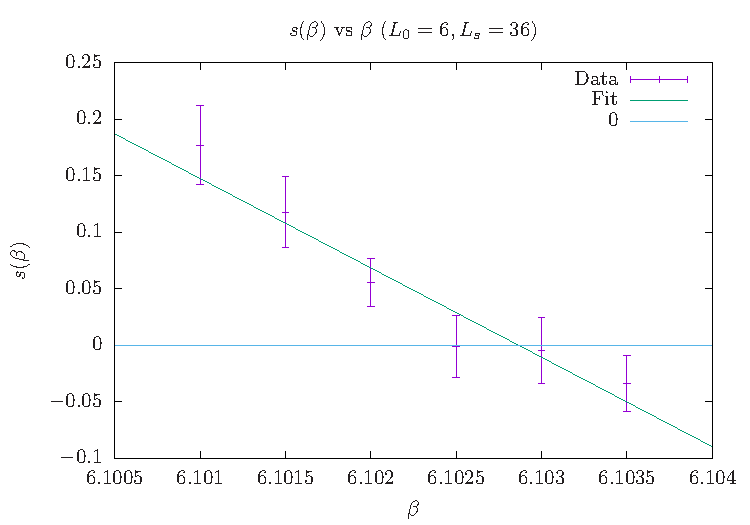
\includegraphics[width=0.45\hsize]{imgs/s_beta.pdf}
    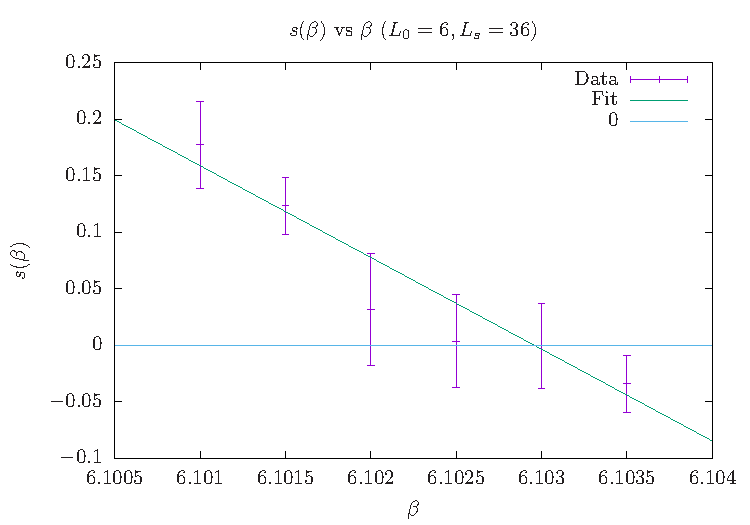
\includegraphics[width=0.45\hsize]{imgs/s_beta_2.pdf}
    
    \caption{(Left) $s(\beta)$ vs $\beta$ using 10 subsamples. $\beta_c = 6.10287(16)$. (Right) $s(\beta)$ vs $\beta$ using 15 subsamples. $\beta_c = 6.10296(20)$}
    \label{fig:beta-crit}
\end{figure}

\newpage
We perform simulations and analyses for 4 different value of $L_0$ from 6 to 9.
In each value of $L_0$, we have computed $s(\beta)$ for some different values of the gauge coupling.
Through a linear fit of these results, we can interpolate the critital value $\beta_{\rm c}$.
In Figures \ref{???}, we plot the $s(\beta)$ against $\beta$ at each $L_0$.
We summarize the value of $\beta_{\rm c}$ at each $L_0$ on Table \ref{???}.

\begin{figure}[h]
    \centering
    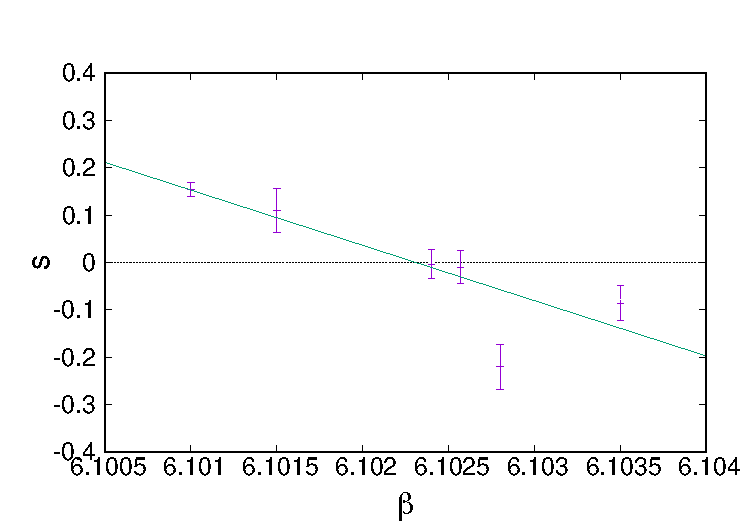
\includegraphics[width=0.3\hsize]{figures/L0_6/plot_s_4pol_Ls_36.pdf}
    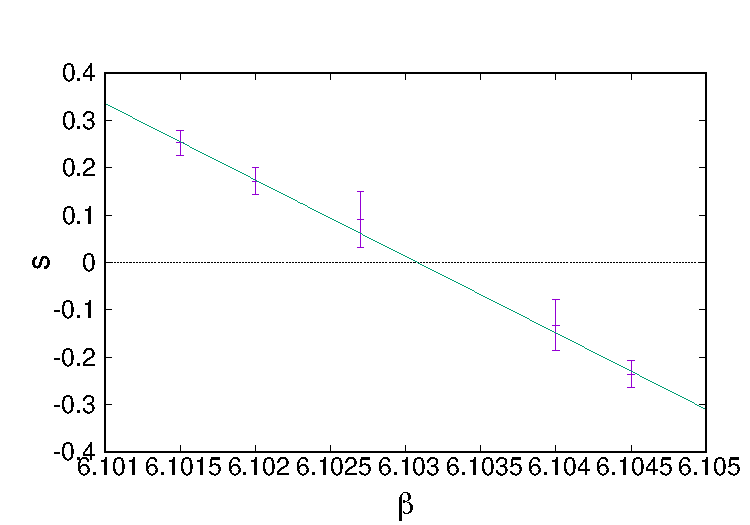
\includegraphics[width=0.3\hsize]{figures/L0_6/plot_s_4pol_Ls_48.pdf}
    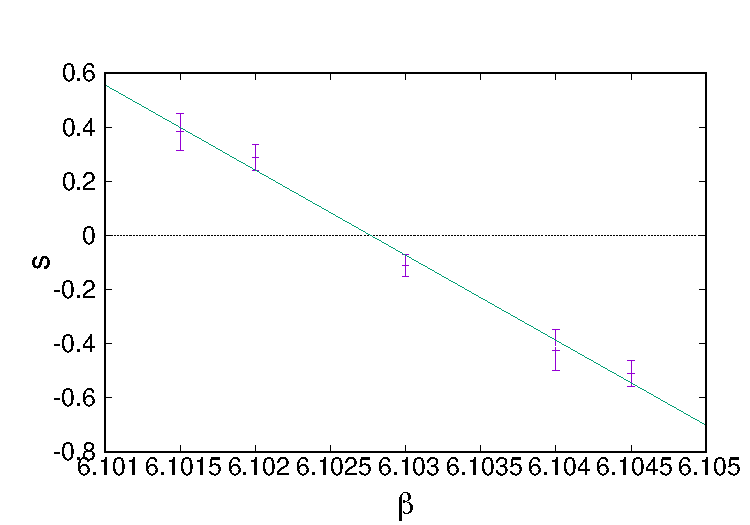
\includegraphics[width=0.3\hsize]{figures/L0_6/plot_s_4pol_Ls_64.pdf}
    \caption{(Left) $L_s=36$, (Middle) $L_s=48$, (Right) $L_s=64$. The results for $L_s=36$ and $L_s=48$ is going to be replaced.}
    \label{fig:L0_6_beta_c}
\end{figure}

\begin{figure}[h]
    \centering
    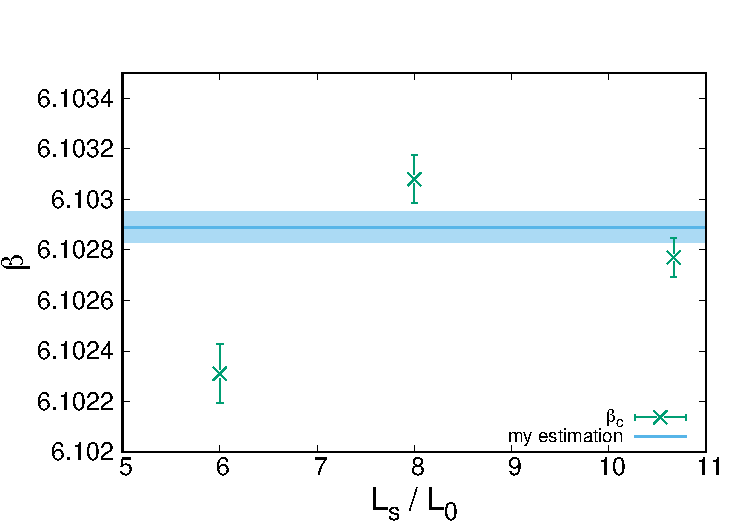
\includegraphics[width=0.5\hsize]{figures/L0_6/vol_dep.pdf}
    \caption{Volume dependence of the $\beta_{\rm c}$ at $L_0 = 6$.}
    \label{fig:L0_6_beta_c_vol}
\end{figure}

\begin{figure}[h]
    \centering
    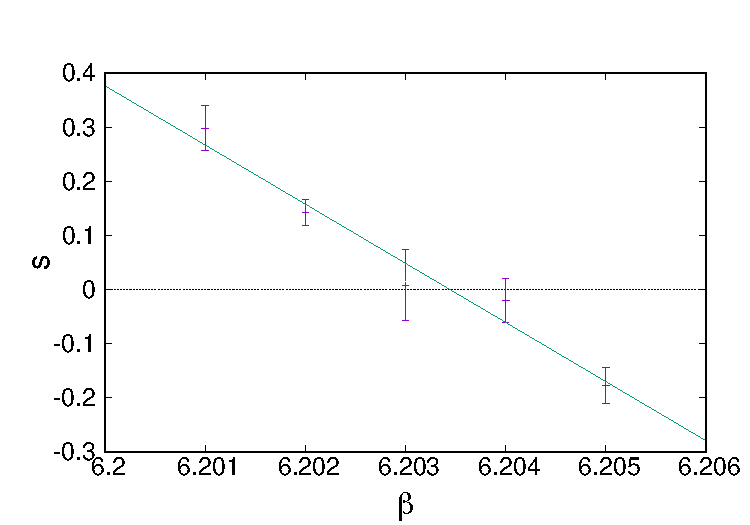
\includegraphics[width=0.33\hsize]{figures/L0_7/plot_s_4pol_Ls_40.pdf}
    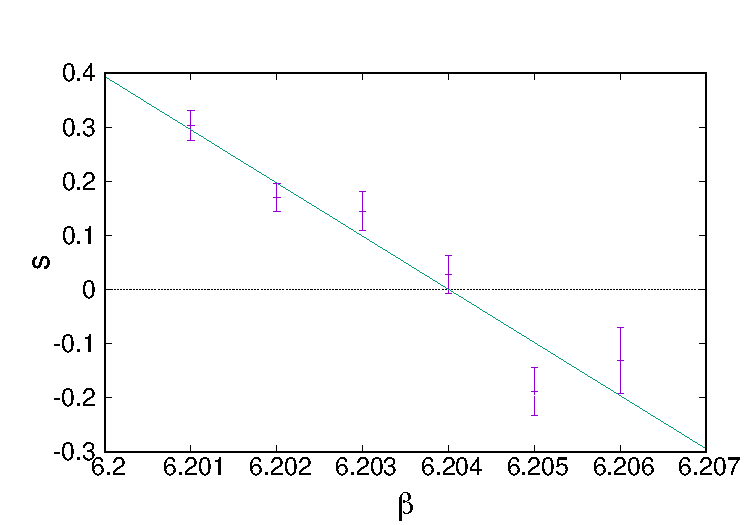
\includegraphics[width=0.33\hsize]{figures/L0_7/plot_s_4pol_Ls_48.pdf}
    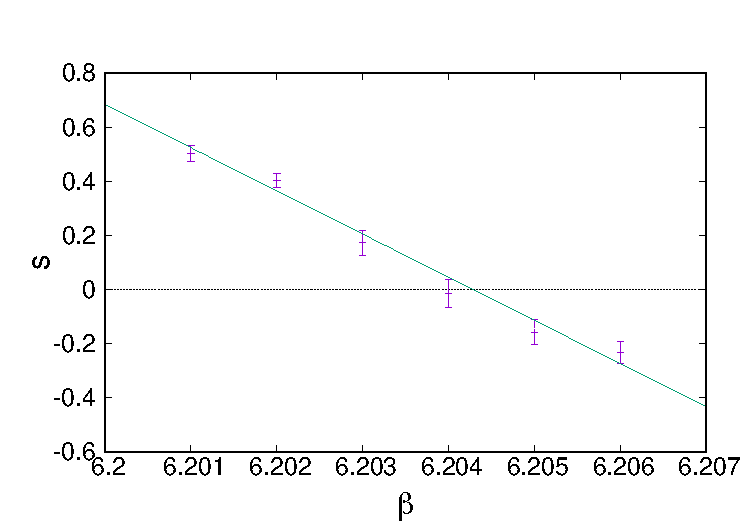
\includegraphics[width=0.33\hsize]{figures/L0_7/plot_s_4pol_Ls_56.pdf}
    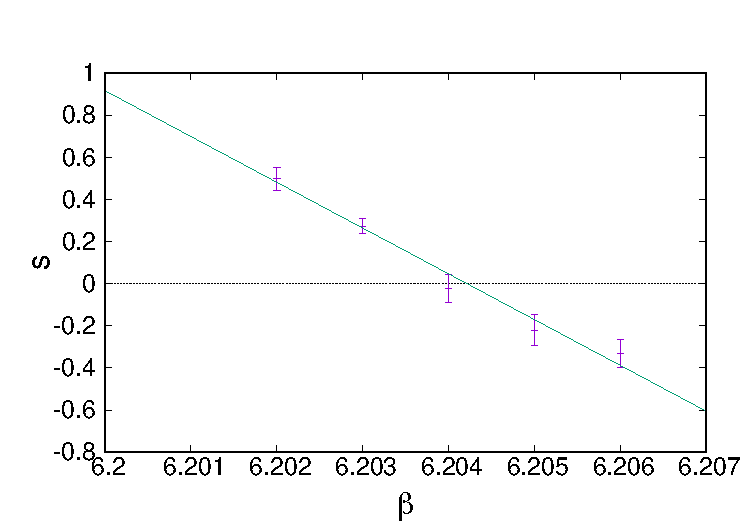
\includegraphics[width=0.33\hsize]{figures/L0_7/plot_s_4pol_Ls_64.pdf}
    \caption{(Left Top) $L_s=40$, (Right Top) $L_s=48$, (Left Top) $L_s=56$, (Right Top) $L_s=64$.}
    \label{fig:L0_7_beta_c}
\end{figure}

\begin{figure}[h]
    \centering
    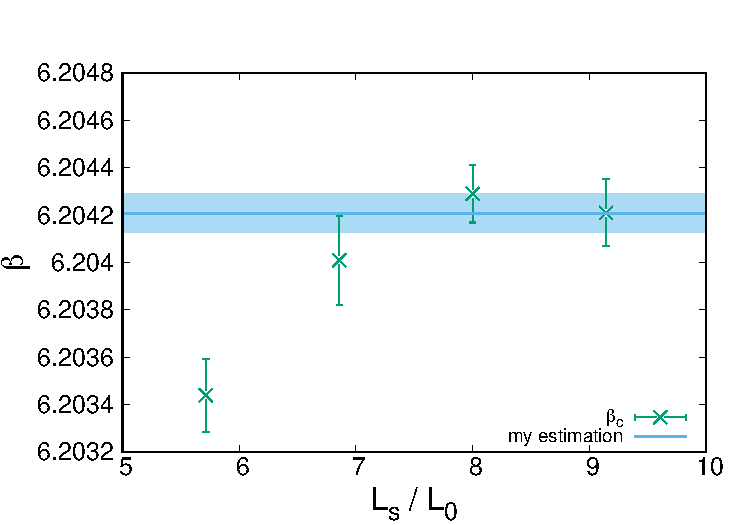
\includegraphics[width=0.5\hsize]{figures/L0_7/vol_dep.pdf}
    \caption{Volume dependence of the $\beta_{\rm c}$ at $L_0 = 7$.}
    \label{fig:L0_7_beta_c_vol}
\end{figure}

\begin{figure}[h]
    \centering
    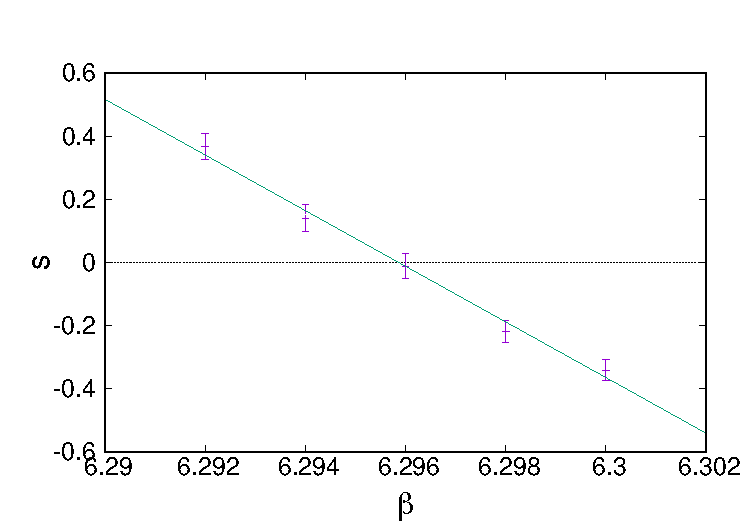
\includegraphics[width=0.33\hsize]{figures/L0_8/plot_s_4pol_Ls_48.pdf}
    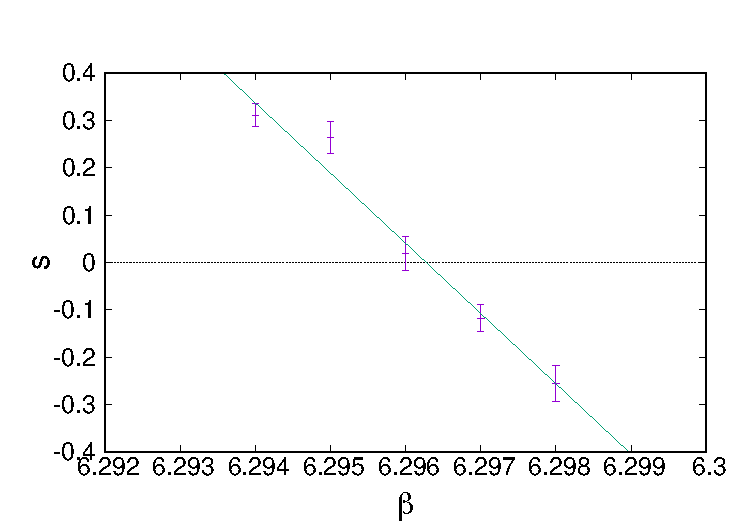
\includegraphics[width=0.33\hsize]{figures/L0_8/plot_s_4pol_Ls_64.pdf}
    \caption{(Left) $L_s=48$, (Right) $L_s=64$}
    \label{fig:L0_8_beta_c}
\end{figure}

\begin{figure}[h]
    \centering
    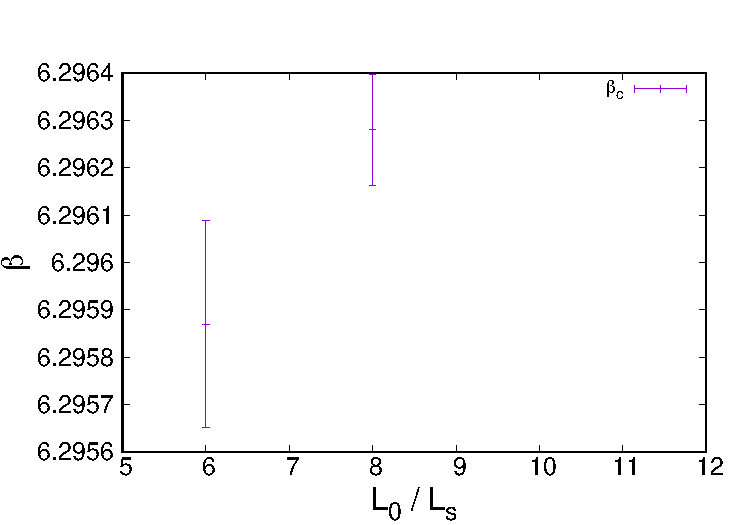
\includegraphics[width=0.5\hsize]{figures/L0_8/vol_dep.pdf}
    \caption{Volume dependence of the $\beta_{\rm c}$ at $L_0 = 8$.}
    \label{fig:L0_8_beta_c_vol}
\end{figure}
\newpage
\section{Measurements of the latent heat}
\begin{figure}[H]
    \centering
    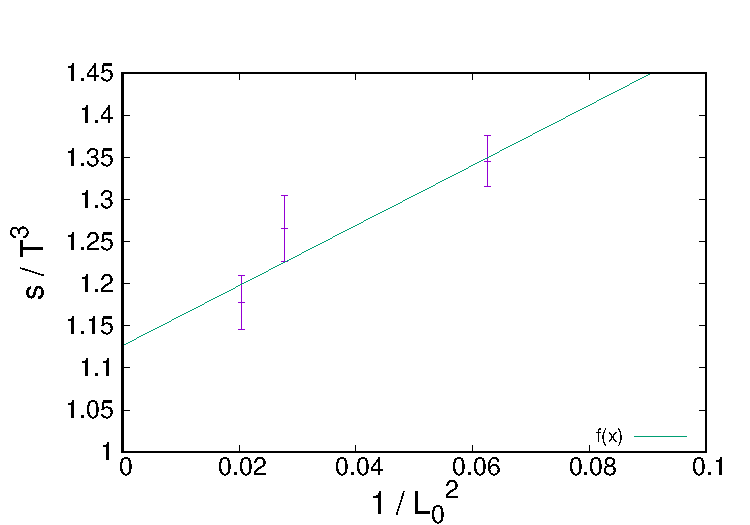
\includegraphics[width=0.5\hsize]{figures/plot_LH_v2.pdf}
    \caption{the latent heat}
    \label{fig:lat_heat}
\end{figure}
\newpage
\section{previous works about the latent heat}

\subsection{Borsanyi et al.}

In this Section we will review some recent results in literature. A similar study for the latent heat of the SU(3) has been conducted by Borsanyi et al. \cite{Borsanyi:2022xml}. In this work the transition temperature has been established through the study of two different observables, namely the susceptibility of the Polyakov Loop:
\begin{equation}
    \chi = N_s^3 \left(\langle \abs{P}^2 \rangle - \langle \abs{P} \rangle^2 \right),
\end{equation}
and the third-order Binder cumulant of $P$:
\begin{equation}
    b_3 = \frac{\langle \abs{P}^3 \rangle - 3 \langle \abs{P} \rangle \langle \abs{P}^2 \rangle + 2 \langle \abs{P} \rangle^3}{\left( \langle \abs{P}^2 \rangle - \langle \abs{P} \rangle^2 \right)^{3/2}}
\end{equation}
Notice that the susceptibility $\chi$ would need to be renormalized in order to compare results from different lattices, but they claim it is not necessary, since $\chi(\beta)$ and $\chi_R(\beta)$ should coincide in the infinite volume limit.

To give a physical expression for the critical temperature, they first define the critical coupling $\beta_c$ through the aforementioned order parameters, then they translate this value into a physical quantity by setting the scale $w_0$ through the Wilson flow method. The latter is implicitly defined by the condition:
\begin{equation}
    t \frac{d}{dt}\left[ t^2 E(t) \right]\rvert_{t = w_0^2
} = 0.3 
\end{equation}
where $E(t)$ is the expectation value of the gauge action computed on gauge configurations evolved via the Wilson flow.
One computes the scale in lattice units $w_0/a(\beta)$ for different couplings on a lattice with fixed temporal extension $L_0$, then the coupling is converted into the dimensionless quantity:
\begin{equation}
    \left(\frac{w_0}{a} \right) \frac{1}{L_0} = w_0 T
\end{equation}
where $T = (a L_0)^{-1}$ is the temperature of the system. The critical coupling $\beta_c$ gets converted into a critical temperature $w_0 T_c$, and by computing this quantity at finite volume for different lattice ratios $L_s/L_0$ one can extrapolate the critical temperature at infinite volume.
From a fit, they found as a final value: $w_0 T_c = 0.25384(23)$.

The latent heat is computed directly as the discontinuity of the trace anomaly $\frac{\Delta(\epsilon - 3p)}{T^4}$ which is encountered as the transition point is crossed.
In practice, the best procedure to compute the latent heat consists in simulating the theory right at the critical coupling $\beta_c$. Throughout a sufficiently long Monte Carlo history, the system will tunnel between gauge configurations both in the cold and hot phase. Given a criterion to separate the two ensembles, they compute the trace anomaly just above and below the cut, and the difference of such values is proportional to the latent heat up to a renormalization factor. As in our case, hot and cold phases are distinguished by studying the distribution of the Polyakov loop expectation value $\langle \abs{P} \rangle$, since these sampling of the phases has systematic errors which decay exponentially with growing volume.

As a final note, one should stress that the trace anomaly suffers from a quartic divergence, which is too computationally costy to make up for by increasing the statistics (it scales with $\sim L_0^8$). To bypass this problem, they adopt a tree-level Symanzik improved action, and they take care of the UV noise of the physical result using a numerical method based on a small gradient flow time evolution.
They define the renormalized trace anomaly as:
\begin{equation}
    \frac{\epsilon - 3p}{T^4} = L_0^4 \, a \, \dv{\beta}{a} \left( \langle S_g \rangle_{L_s^3 \cross L_0} - \langle S_g \rangle_{L_0 = \infty}  \right)
\end{equation}
where $S_g$ is the gauge action in the zero-temperature theory.
Once that the trace anomaly difference has been computed for various lattices, they perform a combined linear continuum and infinite volume fit, leading to the final result:
\begin{equation}
    \Delta \left[ \frac{\epsilon - 3p}{T^4}\right] = 1.025(21)_{\textrm{stat}}(27)_{\textrm{sys}}
\end{equation}
where they quote both the statistical and systematic error.
\printbibliography

\end{document}
